\chapter{Os Métodos de Análise}
\label{chapter:os_metodos_de_analise}

\section{\textbf{K Vizinhos Mais Próximos}}

Link para a figura \ref{fig:knearestneighbors}

\begin{figure}[!htb]
\begin{center}
\caption{K Vizinhos Mais Próximos}
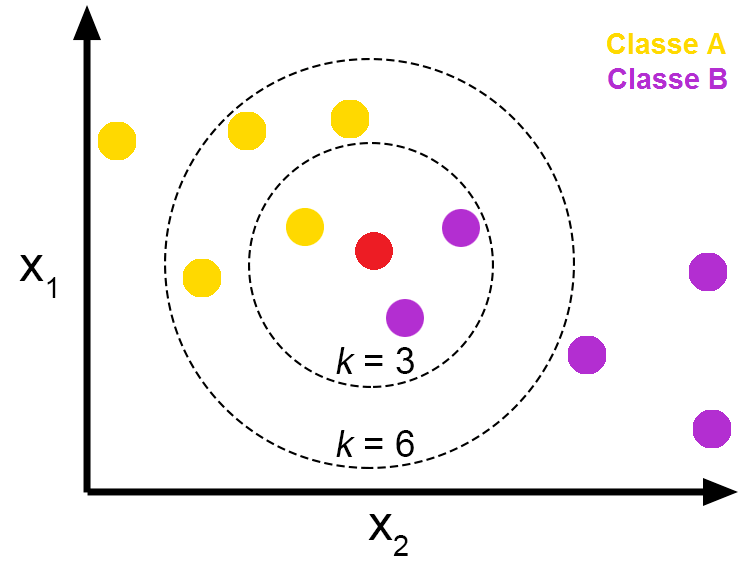
\includegraphics[width=12cm]{knearestneighbors}
\label{fig:knearestneighbors}
\end{center}
\legend{Fonte: \url{https://miro.medium.com/max/1506/0*jqxx3-dJqFjXD6FA} \cite{KNN} }
\end{figure}

\section{\textbf{Árvore de Decisão}}

Figura \ref{fig:decisiontree}

\begin{figure}[!htb]
\begin{center}
\caption{Árvore de Decisão}
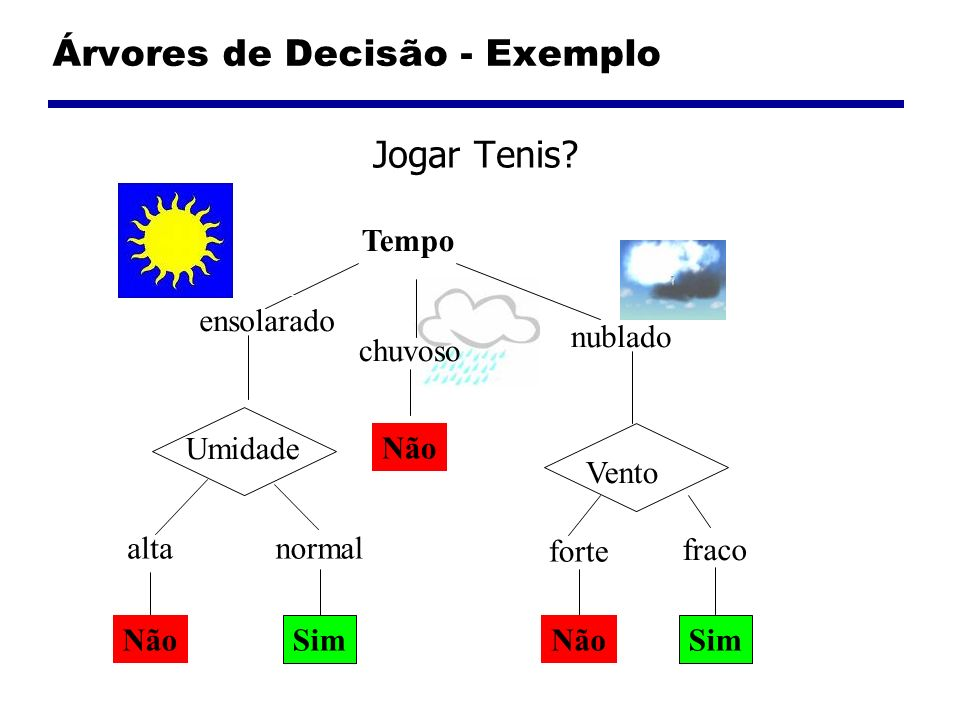
\includegraphics[width=12cm]{decisiontree}
\label{fig:decisiontree}
\end{center}
\legend{Fonte: \url{https://slideplayer.com.br/slide/358847/2/images/5/\%C3\%81rvores+de+Decis\%C3\%A3o+-+Exemplo.jpg}\cite{ARVOREDECISAO}}
\end{figure}


\section{\textbf{Floresta Aleatória}}

Figura \ref{fig:randomforest}.


\begin{figure}[!htb]
\begin{center}
\caption{Floresta Aleatória}
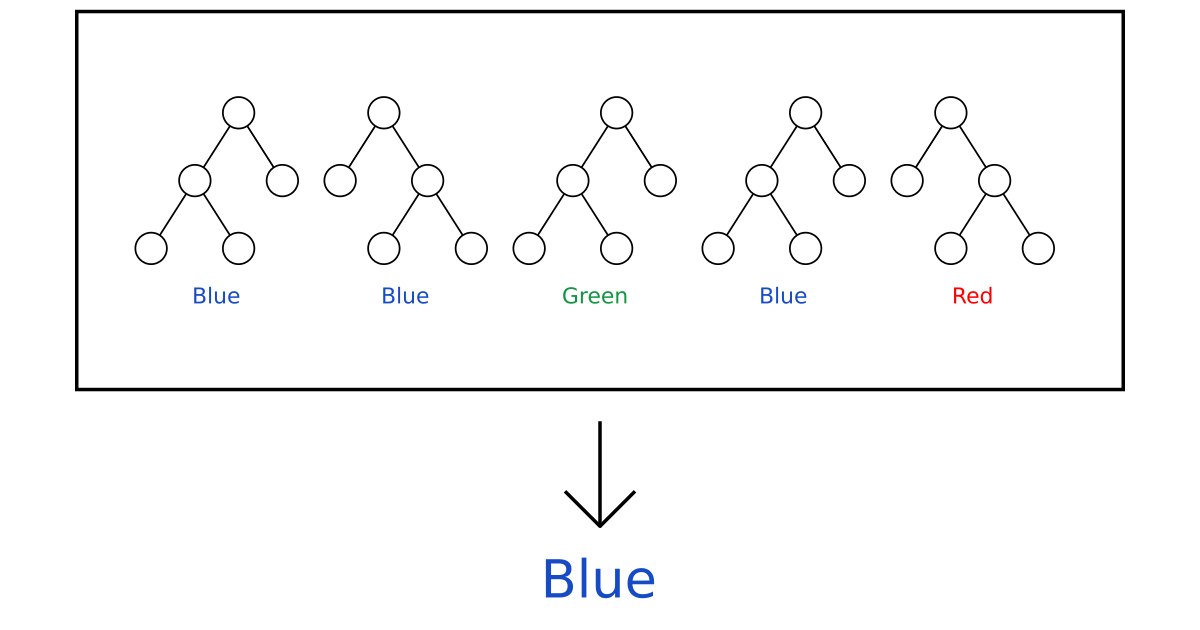
\includegraphics[width=12cm]{randomforest}
\label{fig:randomforest}
\end{center}
\legend{Fonte: \url{https://www.paradigmadigital.com/techbiz/machine-learning-dummies/} \cite{RANDOMFOREST} }
\end{figure}


\section{\textbf{Máquina de Vetor de Suporte}}

Figura \ref{fig:suportvectormachine}

\begin{figure}[!htb]
\begin{center}
\caption{Máquina de Vetor de Suporte}
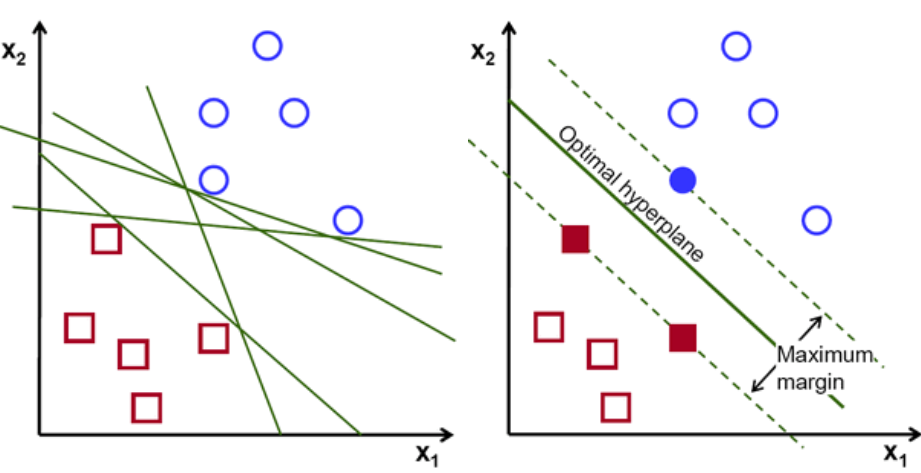
\includegraphics[width=12cm]{suportvectormachine}
\label{fig:suportvectormachine}
\end{center}
\legend{Fonte: \url{https://www.codigofluente.com.br/wp-content/uploads/2019/06/SVM04.png} \cite{SVM} }
\end{figure}

\section{\textbf{Naive bayes}}

\begin{figure}[!htb]
\begin{center}
\caption{Naive Bayes}
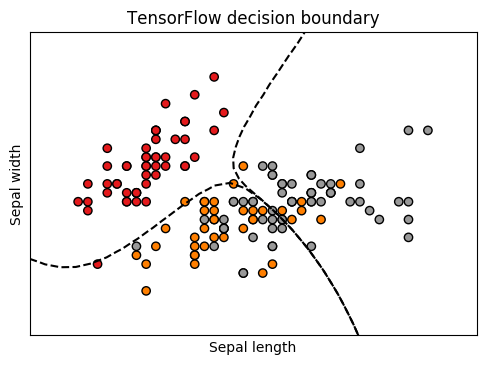
\includegraphics[width=12cm]{naivebayes}
\end{center}
\legend{Fonte: \url{https://www.researchgate.net/profile/Paolo\_Dellaversana/publication/328020065/figure/fig5/AS:677213301121033@1538471641906/Naive-Bayes-classification-of-three-different-rock-types-based-on-nine-mineralogical.png} \cite{NAIVEBAYES} }
\end{figure}

\section{\textbf{Artificial Neural Network}}


\begin{figure}[!htb]
\begin{center}
\caption{Artificial Neural Network}
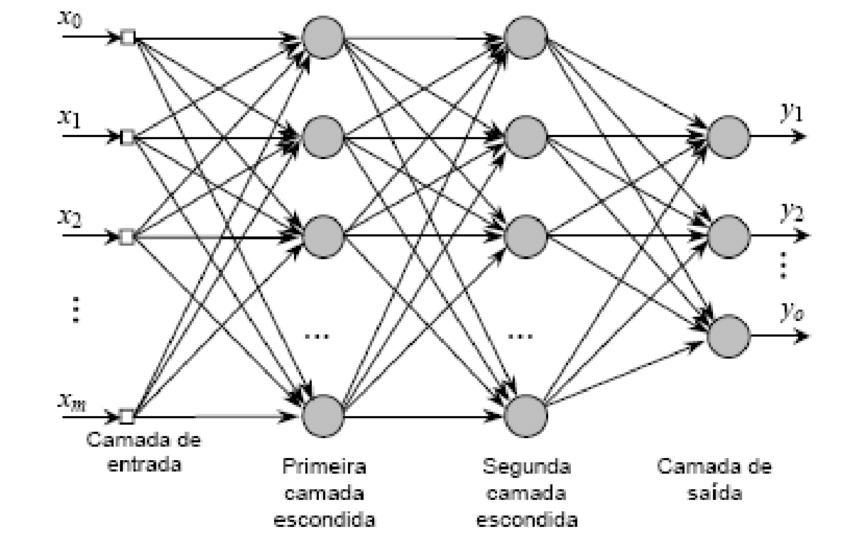
\includegraphics[width=12cm]{mlp}
\end{center}
\legend{Fonte: \url{https://www.researchgate.net/profile/Anderson\_Oliveira6/publication/240772105/figure/fig2/AS:667857415319554@1536241024122/Figura-1-Rede-Neural-Artificial-Multicamadas.png} \cite{MLP} }
\end{figure}


